% Chapter Template

\chapter{Descripci\'on t\'ecnica} % Main chapter title

\label{Chapter3} % Change X to a consecutive number; for referencing this chapter elsewhere, use \ref{ChapterX}

%----------------------------------------------------------------------------------------
%	SECTION 1
%----------------------------------------------------------------------------------------

\section{Descripci\'on t\'ecnica}

\subsection{Aspectos t\'ecnicos de relevancia para los usuarios}
La aplicaci\'on m\'ovil funcionar\'a en dispositivos con Android 5.0, la aplicaci\'on web funcionar\'a en los navegadores Firefox y Chrome. Se necesitar\'a conexi\'on a Internet excepto en el caso de canciones descargadas en la aplicaci\'on m\'ovil. 
\subsection{Aspectos t\'ecnicos de relevancia para el cliente}
\subsubsection{Cluster de prueba}
Se va a desarrollar un protipo funcional de prueba sobre un cluster privado a modo de demostración, se utilizarán sistemas debian y el cluster contar\'a con 5 m\'aquinas entre ellas: un servicio de almacenamiento de 3 m\'aquinas que proporcionar\'an 30 GB protegidos tanto para el repositorio de canciones como para almacenarlas m\'aquinas virtuales, un servidor que exporta el almacenamiento por HTTP y un servidor de virtualización con la web, el backend y la base de datos.
\subsubsection{Entrega al cliente}
Se entregar\'a al cliente las instrucciones, c\'odigos y software necesario para poder replicar la instalaci\'on identica en su cluster privado. Adem\'as se le dar\'a acceso al cluster de pruebas donde podr\'a probar la infrastructura.
\subsection{Descripci\'on t\'ecnica preliminar}
El sistema cuenta con 4 componentes principales: una aplicaci\'on Android, una aplicaci\'on web, un servidor web (a modo de coordinaci\'on) y un sistema de almacenamiento.
El servidor web ser\'a una sola m\'aquinas con sistema operativo ProxmoxVE(basado en Debian), contar\'a con 2 m\'aquinas virtuales,un sistema gestor de bases de datos PostgreSQL y una aplicaci\'on backend en Tomcat para la web est\'atica y el servidor REST backend. Ambas m\'aquinas residen en el servicio de almacenamiento mediante RBD, esto permite garantizar la integridad de los datos mediante replicaci\'on y en el caso de disponer de varias m\'aquinas para virtualizar permitir configurar tolerancia a fallos y migrados de m\'aquinas.
El servicio de almacenamiento ser\'a un conjunto de 4 m\'aquinas, 3 ceph-nodes que ofrecen el almacenamiento, replica, distribuci\'on y consistencia de los datos y una cuarta, ceph\_rados\_gw que ofrece una interfaz REST mediante HTTP para el acceso a los datos equiparable a Amazon S3 o Swift. Todas las canciones y datos disponen de un URI.
Las comunicaciones con el cliente se realizar\'an siempre mediante HTTP con una interfaz RESTfull. El cliente se comunicar\'a con la aplicaci\'on Tomcat en caso de necesitar consultar valores o actualizar la base de datos y en cambio se comunicar\'a directamente con el servidor RADOS para obtener las canciones, esta separaci\'on permite no sobrecargar al servidor de Tomcat ni a su red con descargas de datos pesados.
Para soportar la integridad de los datos, el servicio de almacenamiento con 3 m\'aquinas permite una ca\'ida de 1 m\'aquina simultanea sin p\'erdida de servicio.

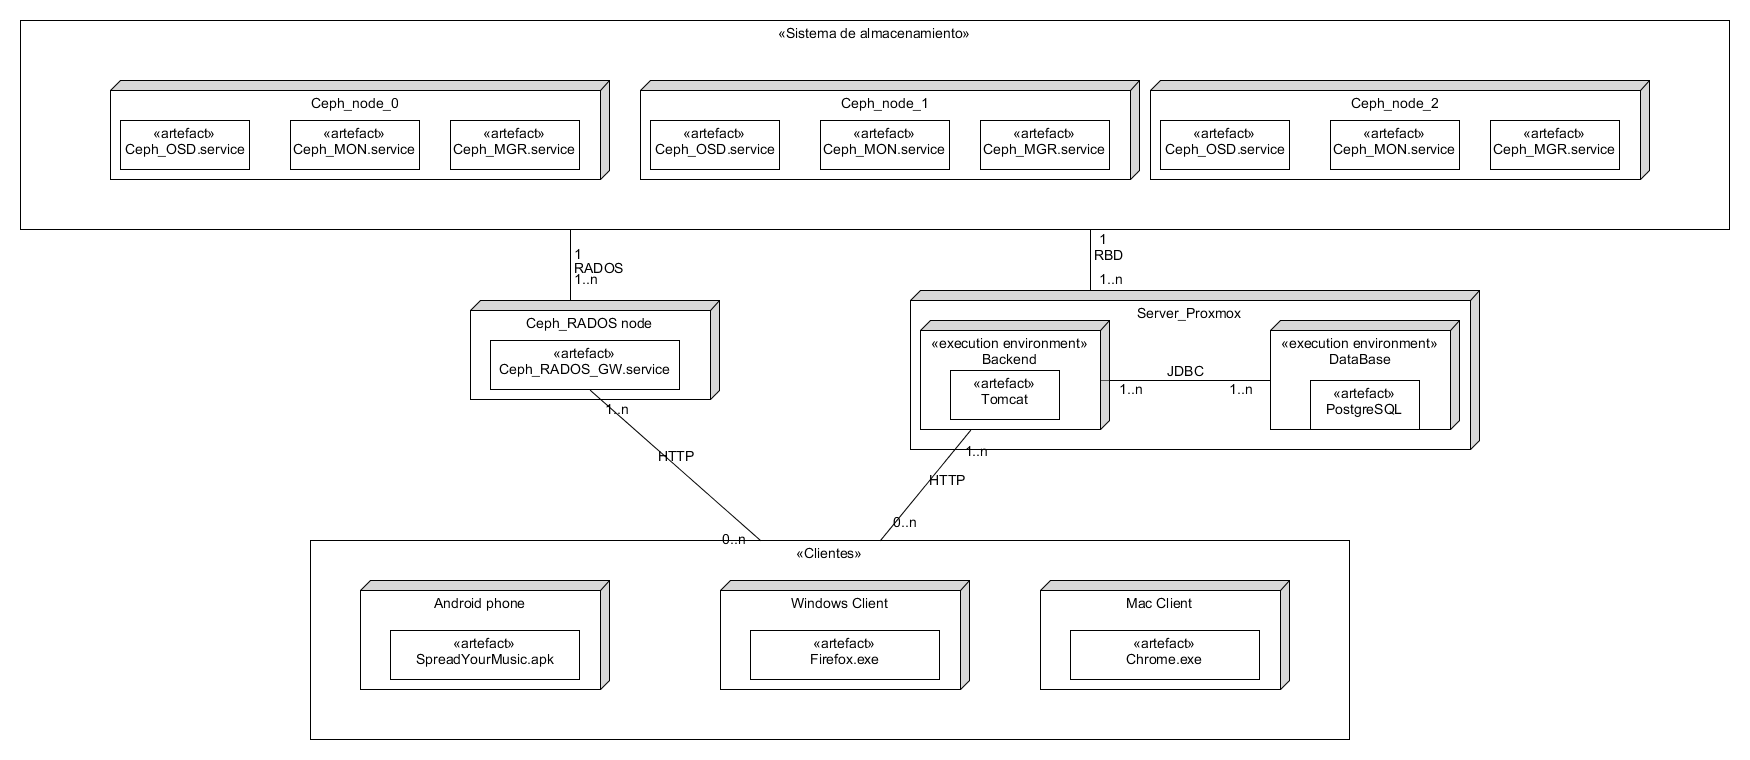
\includegraphics[width=\textwidth]{Figures/deployment.png}